\begin{enumerate}[label=(\alph*)]
\item Khi vôn kế được chuyển sang vị trí 1, điện áp trên que graphite sẽ được đo, trong khi ở vị trí 2, điện áp đo được là điện áp trên điện trở 1.0 $\Omega$. Nếu điện áp được đo bằng vôn, thì điện áp trên điện trở sẽ bằng với cường độ dòng điện trong mạch tính bằng ampe. Ở đây, ta nên sử dụng điện trở 1.0 $\Omega$ thay vì 10 $\Omega$ để thuận tiện cho việc đọc số liệu.
\item Từ bảng số liệu, ta thu được đồ thị sau: 
\begin{figure}[H]
    \centering
        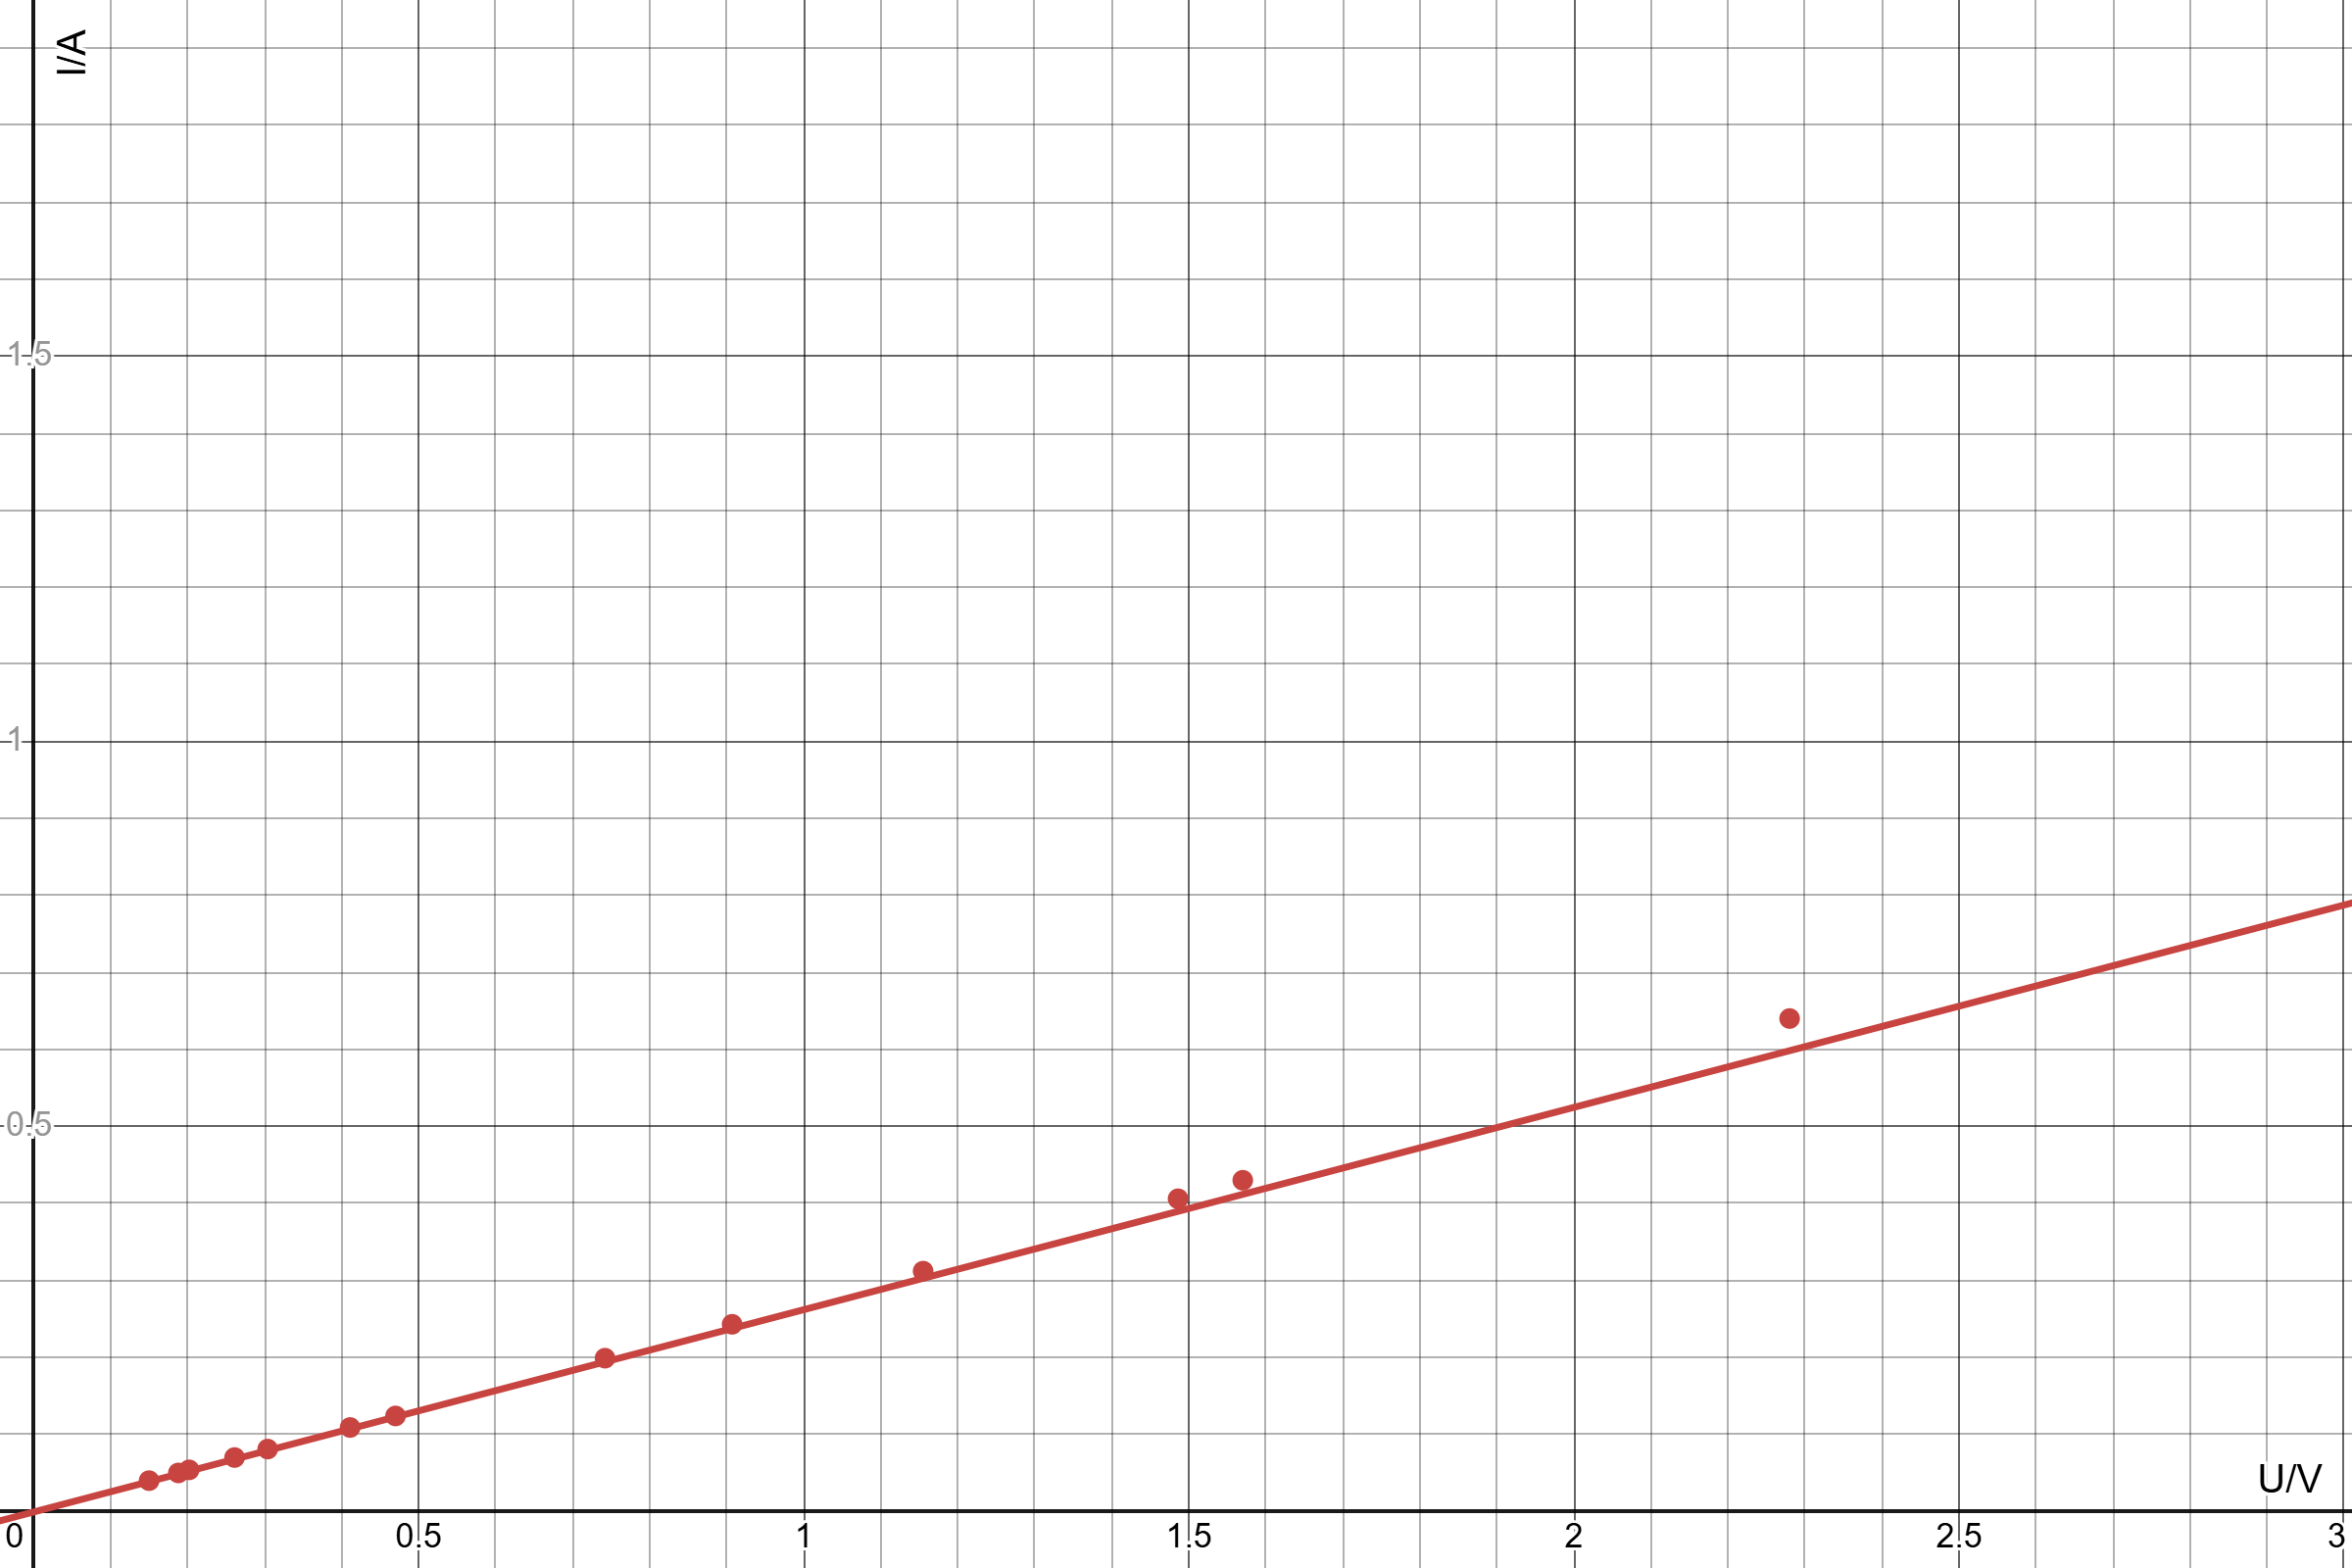
\includegraphics[scale=0.15]{Problem_3/Figs_P3/ExpSol1.PNG}
    \caption{}
    \label{fig:S3_01}
\end{figure}
\item Trong trạng thái cân bằng, ta viết được phương trình cân bằng nhiệt: 
\begin{equation}
\dfrac{U^2}{R_0(1 + \alpha \Delta T)} = \beta \Delta T.
\end{equation}
Giải phương trình bậc hai cho sự chênh lệch nhiệt độ dẫn đến
\begin{align}
\frac{U^2}{R_0} &= \beta \Delta T (1 + \alpha \Delta T) \Rightarrow \alpha \beta (\Delta T)^2 + \beta \Delta T - \frac{U^2}{R_0} = 0. \\
\Delta T &= \frac{-\beta \pm \sqrt{\beta^2 + 4 \frac{U^2}{R_0} \alpha \beta}}{2\alpha \beta}.
\end{align}
Từ dữ liệu thu được suy ra rằng hệ số nhiệt độ của điện trở graphit là âm, do đó nghiệm nhỏ hơn sẽ là nghiệm với dấu + . Do đó, phương trình mô tả đặc tính U-I lý thuyết có dạng:
\begin{equation}
I = \dfrac{U}{R_0(1 + \alpha \Delta T)} = \dfrac{U}{R_0\left(1 + \frac{-\beta + \sqrt{\beta^2 + 4 \frac{U^2}{R_0} \alpha \beta}}{2\beta}\right)} \approx \frac{U}{R_0\left(1 + \frac{U^2}{R_0} \frac{\alpha}{\beta}\right)} \approx \frac{U}{R_0} \left[1 - \frac{U^2}{R_0} \frac{\alpha}{\beta}\right].
\end{equation}
\item Từ số liệu thí nghiệm đã cho, ta tính được điện trở của miếng graphite: $R_0=3.78 \Omega$. Để chính xác nhất có thể, ta se chỉ xử lý những số liệu thu được ở giá trị điện thế thấp (<0.5V) vì ở thời điểm đó, thanh graphite sẽ chưa bị nóng lên quá nhiều.\\
Điện trở suất của miếng graphite: \\
\begin{equation}
\boxed{
    \rho=\dfrac{\pi d^2}{4l}R_0=5.93 \cdot 10^{-5} \left( \Omega\cdot \si{m}\right).
    }
\end{equation}
\item Trong trạng thái cân bằng, công suất tỏa ra khi dòng điện chạy qua bằng với công suất tổn hao nhiệt:
\begin{equation}
P = \beta \Delta T \quad \Rightarrow \quad \Delta T = \frac{P}{\beta}.
\end{equation}
Do đó, sự phụ thuộc của điện trở vào công suất có dạng:
\begin{equation}
\boxed{
R_g = R_0(1 + \alpha \Delta T) = R_0\left(1 + \dfrac{\alpha}{\beta} P\right).
}
\end{equation}
\item Sự phụ thuộc của điện trở vào công suất tiêu tốn được biểu diễn trong hình vẽ.
\begin{figure}[H]
    \centering
    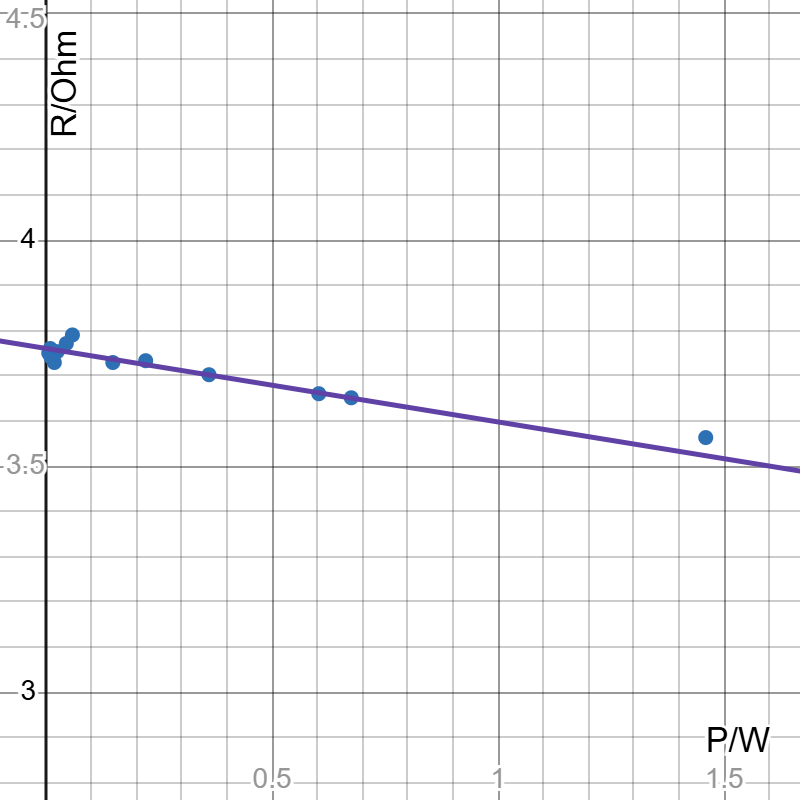
\includegraphics[scale=0.45]{Problem_3/Figs_P3/ExpSol2.PNG}
    \caption{}
    \label{fig:S3_02}
\end{figure}
Tính tuyến tính của sự phụ thuộc này được quan sát thấy ở các công suất lớn hơn $0,2W$. \\
Đặt biểu thức biểu diễn sự phụ thuộc tuyến tính giữa R và P là $R = aP + b$. Từ đồ thị, ta tính xấp xỉ được $a = 0.16 \Omega \cdot W^{-1}$, $b = 3.76 \Omega$, do đó, hệ số $\gamma$ trong công thức ở phần (e) được tính như sau: \\
\begin{equation}
\boxed{
\gamma = \frac{a}{b} = 0.035 \left(\si{W}^{-1}\right).
}
\end{equation}
\newpage 
\item Từ bảng số liệu đã cho, ta vẽ được đồ thị như sau: 
\begin{figure}[H]
    \centering
    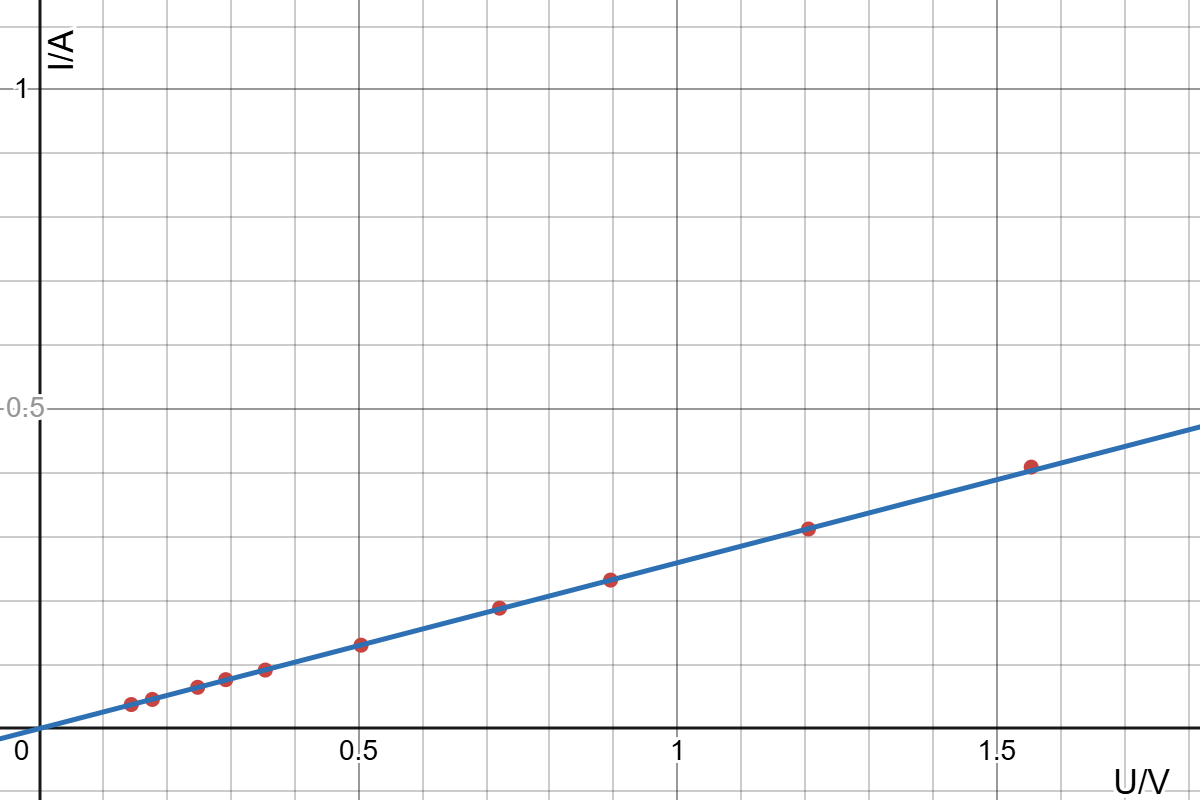
\includegraphics[scale=0.4]{Problem_3/Figs_P3/ExpSol3.PNG}
    \caption{}
    \label{fig:S3_03}
\end{figure}
Trong đồ thị này cũng có một sự phi tuyến tính nhỏ khi công suất tăng. Do đó, để tính điện trở ở nhiệt độ không, chỉ nên sử dụng một vài điểm ban đầu với điện trở thấp. Tính toán cho năm điểm đầu tiên dẫn đến giá trị sau:
\begin{equation}
R_g = 3.88 \left(\Omega\right).
\end{equation}
Vì giá trị này phải tuân theo công thức $R_g = R_0(1 + \alpha \Delta T)$, hệ số nhiệt độ của điện trở có thể được tính như sau:
\begin{equation}
\boxed{
\alpha = \frac{1}{\Delta T} \left(\frac{R_g}{R_0} - 1\right)= -1.3 \cdot 10^{-3} \left(\si{K}^{-1}\right).
}
\end{equation}
\newpage
\textbf{Phổ điểm}
    \begin{center}
    \begin{tabular}{|c|p{8cm}|c|}
    \hline
    \multicolumn{1}{|l|}{Phần} & Nội dung & Điểm thành phần \\ 
    \hline
\multirow{1}{*}{(a)} & Giải thích đúng cách đo.                                                                                  & 0.25             
                                \\ \hline
\multirow{1}{*}{(b)} & Vẽ đúng đồ thị.                                                                                & 0.25             
                                \\ \hline
\multirow{4}{*}{(c)} & Viết đúng phương trình cân bằng nhiệt.                               
                     & 0.25            \\ \cline{2-3}
                     & Giải đúng phương trình bậc 2 cho sự chênh lệch nhiệt độ.         
                     & 0.25            \\ \cline{2-3}
                     & Chọn đúng nghiệm nhỏ hơn                
                     & 0.25            \\ \cline{2-3}
                     & Viết đúng biểu thức cuối của I theo các đại lượng              
                     & 0.25           
                     \\ \hline
\multirow{2}{*}{(d)} & Xử lý được số liệu và thu được điện trở miếng graphite (cho phép sai số $0.03\Omega$)                            
                     & 0.5            \\ \cline{2-3}
                     & Tính được đúng điện trở suất từ điện trở đã được tính được    
                     & 0.25             
                     \\ \hline
\multirow{1}{*}{(e)} & Viết đúng biểu thức $R_g$                                                                            & 0.25          
\\ \hline     
\multirow{2}{*}{(f)} & Vẽ được đồ thị chuẩn                                                                        & 0.25    \\ \cline{2-3}     
& Từ đồ thị xấp xỉ được hai giá trị a và b và tính được $\gamma$                                                   & 0.5  
                                \\ \hline
\multirow{1}{*}{(g)} & Vẽ được đồ thị chuẩn                                                                        & 0.25     \\ \cline{2-3}     
& Từ đồ thị tính được $R_g$                                                   
& 0.25     \\ \cline{2-3}
& Tính được đúng giá trị của $\alpha$                                                   
& 0.25     \\ \hline                                


    \end{tabular}
    \end{center}
\end{enumerate}